\documentclass[a4paper,11pt]{article}

%%%%%%%%%%%%%%%%%%%%%%%%%%%%%%%%%%%%%%%%%%%%%%%%%%%%%%%%%%%%%%%%%%%%%%%%
% Paquetes utilizados
%%%%%%%%%%%%%%%%%%%%%%%%%%%%%%%%%%%%%%%%%%%%%%%%%%%%%%%%%%%%%%%%%%%%%%%%

% Gráficos complejos
\usepackage{graphicx}
\usepackage{caption}
\usepackage{subcaption}
\usepackage{placeins}

% Soporte para el lenguaje español
\usepackage{textcomp}
\usepackage[utf8]{inputenc}
\usepackage[T1]{fontenc}
\DeclareUnicodeCharacter{B0}{\textdegree}
\usepackage[spanish]{babel}

% Código fuente embebido
\usepackage{listings}

% PDFs embebidos para el apéndice
\usepackage{pdfpages}

% Matemáticos
\usepackage{amssymb,amsmath}

% Tablas complejas
\usepackage{multirow}

% Formato de párrafo
\setlength{\parskip}{1ex plus 0.5ex minus 0.2ex}

%%%%%%%%%%%%%%%%%%%%%%%%%%%%%%%%%%%%%%%%%%%%%%%%%%%%%%%%%%%%%%%%%%%%%%%%
% Título
%%%%%%%%%%%%%%%%%%%%%%%%%%%%%%%%%%%%%%%%%%%%%%%%%%%%%%%%%%%%%%%%%%%%%%%%

% Título principal del documento.
\title{\textbf{Trabajo Práctico 1: Conjunto de Instrucciones MIPS}}

% Información sobre los autores.
\author{\\
  Guido Laghi, \textit{P. 82.449}                                  \\
  \texttt{guido321@gmail.com}                                      \\ [2.5ex]
  Sebastián L. Pérez, \textit{P. 84.379}                           \\
  \texttt{sebastian.leo.perez@gmail.com}                           \\ [2.5ex]
  Sergio Matías Piano, \textit{P. 85.191}                          \\
  \texttt{smpiano@gmail.com}                                       \\ [2.5ex]
                                                                   \\
  \normalsize{1er. Cuatrimestre de 2013}                           \\
  \normalsize{66.20 Organización de Computadoras}                  \\
  \normalsize{Facultad de Ingeniería, Universidad de Buenos Aires} \\
}
\date{}

%%%%%%%%%%%%%%%%%%%%%%%%%%%%%%%%%%%%%%%%%%%%%%%%%%%%%%%%%%%%%%%%%%%%%%%%
% Documento
%%%%%%%%%%%%%%%%%%%%%%%%%%%%%%%%%%%%%%%%%%%%%%%%%%%%%%%%%%%%%%%%%%%%%%%%

\begin{document}

% ----------------------------------------------------------------------
% Top matter
% ----------------------------------------------------------------------
\thispagestyle{empty}
\maketitle

\begin{abstract}

  Este informe sumariza el desarrollo del trabajo práctico 1 de la materia
  Organización de Computadoras (66.20) dictada en el primer cuatrimestre de
  2013 en la Facultad de Ingeniería de la Universidad de Buenos Aires. El mismo
  consiste en la construcción de un sistema minimalista de ordenamiento de
  archivos y el análisis de performance y perfilado del mismo.

\end{abstract}

\clearpage

% ----------------------------------------------------------------------
% Tabla de contenidos
% ----------------------------------------------------------------------
\tableofcontents
\clearpage


% ----------------------------------------------------------------------
% Desarrollo
% ----------------------------------------------------------------------
\part{Desarrollo}

\section{Introducción}

El proceso de compilación de un programa codificado en C consiste en un
pipeline que genera finalmente código objeto para una arquitectura objetivo.
Este pipeline analiza y traduce el código a diferentes representaciones de los
algoritmos contenidos en él, de manera de terminar generando código objeto que
finalmente se linkea en un ejecutable válido para la arquitectura.

Debido a que el lenguaje C es un lenguaje de alto nivel, varios de los
conceptos propios de este lenguaje deben ser mapeados a diferentes estrategias
que pueden ser ejecutadas en el código objeto, que no es más que el conjunto de
instrucciones que la arquitectura objetivo provee. Estos mapeos muchas veces
pueden implementarse de diferentes maneras, cada una con sus ventajas y
desventajas, y si bien el compilador realiza una muy buena tarea en determinar
la mejor manera en la que traducir estos conceptos en instrucciones de bajo
nivel, los algoritmos utilizados no garantizan que la traducción sea de manera
de generar el código objeto más eficiente y compacto que se podría tener.

La alternativa que se propone explorar en el presente trabajo es la
implementación directa en assembly de las rutinas del sistema que se está
construyendo. Esta alternativa tiene una característica fundamental: al tener
acceso al conjunto de instrucciones que ejecuta la arquitectura potencialmente
se puede desarrollar una solución óptima, minimizando el acceso a memoria, la
cantidad de instrucciones a ejecutar, etc.

Por otro lado, la implementación en assembly de un sistema no trivial es una
tarea complicada. La dificultad principal radica en que es tarea del
programador implementar y controlar muchos de los mecanismos de bajo nivel que
constituyen el \textit{cómo} de la solución, en vez de concentrarse en el
\textit{qué}. Algunos ejemplos son el manejo del stack, la implementación de
convenciones de llamadas de subrutinas, el uso de registros compartidos, entre
otros.

\section{Implementación}

El sistema que resuelve el problema planteado en el enunciado (disponible en el
anexo \ref{sec:enunciado}) fue implementado mayoritariamente en C, y parte en 
lenguaje MIPS como lo indicaba el enunciado. La diferencia fundamental radica 
en la implementación de las rutinas de ordenamiento a través del algoritmo 
\textit{shellsort} directamente en assembly. El código fuente de
la solución está disponible en el anexo \ref{sec:source}; por cuestiones de
espacio y prolijidad sólo se incluyen los archivos relacionados con la
implementación en assembly de la solución desarrollada.

Cabe destacar que la solución en assembly definitivamente no es la solución
óptima. Existen algunas mejoras posibles para disminuir la cantidad de
instrucciones a ejecutar o los accesos a memoria: por ejemplo, se podrían
reordenar las instrucciones de algunos de los bloques de los procedimientos
implementados para eliminar algunas de las instrucciones de salto
incondicional, o se podrían utilizar de mejor manera los registros salvados
(s0-s8) para eliminar la necesidad de restaurar desde el stack algunos de los
registros en uso (particularmente a0, a1 y a2 en la implementación de
\textit{shell\_sort\_s}). Sin embargo, dado que la solución que se presenta
contiene el \(40\%\) de las instrucciones del equivalente implementado en C
compilado sin optimizaciones, a los efectos del trabajo práctico consideramos
suficientemente óptima la implementación propuesta.

A continuación enumeraremos algunas consideraciones de diseño tomadas al
implementar cada una de las funciones involucradas en el algoritmo de
ordenamiento.

\subsection{shell\_sort\_s}

Esta función implementa el ordenamiento de una tabla de strings a través de
\textit{shellsort}. El método de ordenamiento fue implementado en su forma más
sencilla a través de un algoritmo recursivo. El stack frame típico de la
función se describe en la imagen adjunta al final del informe.

\FloatBarrier

Se reservan 32 bytes para el área de SRA: 4 bytes para salvar el registro ra en llamadas a otras funciones (ya que no es leaf), 4 bytes para salvar el registro gp, 4 bytes para preservar el registro fp y finalmente 20 bytes para el uso interno de los registros S0, S1, S2, S3, S4 que se utilizan para cálculos de la función.

Por otro lado, dado que las funciones invocadas desde esta no poseen nunca más
de dos argumentos, se reservan \(4 x 4\) bytes en concepto de ABA (respetando la ABI) para ser

utilizados por las funciones llamadas.

Esta función invoca a strcasecmp como a data\_swaper.

\FloatBarrier

\section{Compilación}

Se instrumentó un \textit{makefile} para ejecutar las instrucciones adecuadas
de compilación para los distintos escenarios requeridos. La
tarea \textit{make} compila individualmente cada uno de los archivos fuente de
extensión \textit{c} y \textit{S} a través del ejecutable \textit{gcc}.
Los comandos utilizados para compilar cada uno de estos archivos fuente son los
siguientes:

\begin{lstlisting}
gcc -c -o build/obj/buffer.o source/buffer.c -I./source -Wall 
gcc -c -o build/obj/data.o source/data.c -I./source -Wall 
gcc -c -o build/obj/clargs.o source/clargs.c -I./source -Wall 
gcc -c -o build/obj/cltext.o source/cltext.c -I./source -Wall 
gcc -c -o build/obj/tp1.o source/tp1.c -I./source -Wall 
gcc -c -o build/obj/bubblesort.o source/bubblesort.c -I./source -Wall 
gcc -c -o build/obj/shellsort.o source/shellsort.c -I./source -Wall 
\end{lstlisting}

De este listado, cada una de las invocaciones obedece a la siguiente estructura
de argumentos:

\begin{description}

  \item[-c] Compila o ensambla el código fuente pero no corre el linker.  Por
    lo tanto la salida corresponde a un archivo objeto por cada archivo fuente.

  \item[-o] Especifica cual será el archivo de salida sea éste un archivo
    objeto, ejecutable, ensamblado o código preprocesado de C.

  \item[-Wall] Activa todos los mensajes de warning.

  \item[-I] Agrega el directorio especificado a la lista de directorios
    buscados para los archivos header

\end{description}

El resultado de la ejecución de estos comandos es que se generan archivos
objeto para cada fuente, listos para ser linkeados, en el directorio
\textit{build/obj}. Para realizar este último paso, se invoca nuevamente a
\textit{gcc} con un último comando:

\begin{lstlisting}
gcc -o build/tp1 build/obj/buffer.o build/obj/data.o build/obj/clargs.o build/obj/cltext.o build/obj/tp1.o build/obj/bubblesort.o build/obj/shellsort.o -I./source -Wall 
\end{lstlisting}

El comando linkea todos los archivos objeto en un ejecutable final,
\textit{build/tp1}.

\section{Análisis de tiempos de ejecución}

En las siguientes secciones detallaremos el proceso de análisis de tiempo de
ejecución realizado para los diferentes casos contemplados.

\subsection{Análisis previo}\label{sec:tiempos}

El análisis de tiempos de ejecución se focalizará en comparar la performance de
la implementación en assembly descripta anteriormente contra diferentes
versiones de esencialmente el mismo sistema.

Primero se comparará el desempeño de los algoritmos escritos en C. utilizando todas las optimizaciones disponibles por el
compilador. Se espera nuevamente encontrar algunas mejoras, aunque pequeñas,
con respecto a lo que puede entregar el compilador.

Luego se comparará el algoritmo escrito en C contra el mismo en lenguaje ensabmblador.
Por un lado, al compilar esta solución sin ninguna optimización del compilador 
se espera obtener ganancias de performance apreciables, debidas mayormente al 
mejor manejo de los accesos a memoria logrados por el ejecutable desarrollado en assembly.

\subsection{Experimentos}

Se realizaron pruebas utilizando los archivos provistos por la cátedra sobre un entorno de ubuntu actual y sobre el emulador GXemul.
Obtuvimos los siguientes resultados:

\begin{table}[h!t]
\centering
\begin{tabular}{ | l | r | }
  \hline
  Archivo          & Tiempo de ejecución \\ \hline
  Alice				 & \(13.107s\) \\
  Beowulf     & \(20.749s\) \\
  Cyclopedia     & \(3m 27.744s\) \\
  EL Quijote      & \(60m 32.782s\) \\
  \hline
\end{tabular}
\caption{Tiempos en Ubuntu para BubbleSort}
\label{tab:resultados}
\end{table}

\FloatBarrier

\begin{table}[h!t]
\centering
\begin{tabular}{ | l | r | }
  \hline
  Archivo          & Tiempo de ejecución \\ \hline
  Alice				 & \(0.422s\) \\
  Beowulf     & \(0.537s\) \\
  Cyclopedia     & \(1.920s\) \\
  EL Quijote      & \(5.675s\) \\
  \hline
\end{tabular}
\caption{Tiempos en Ubuntu para ShellSort}
\label{tab:resultados}
\end{table}

\FloatBarrier

\begin{table}[h!t]
\centering
\begin{tabular}{ | l | r | }
  \hline
  Archivo          & Tiempo de ejecución \\ \hline
  Alice				 & \(15m 17.180s\) \\
  Beowulf     & \(27m 11.102s\) \\
  Cyclopedia     & \(135m\) \\
  EL Quijote      & \(time elapsed\) \\
  \hline
\end{tabular}
\caption{Tiempos en GXemul para BubbleSort}
\label{tab:resultados}
\end{table}

\FloatBarrier

\begin{table}[h!t]
\centering
\begin{tabular}{ | l | r | }
  \hline
  Archivo          & Tiempo de ejecución \\ \hline
  Alice				 & \(7.281s\) \\
  Beowulf     & \(9.500s\) \\
  Cyclopedia     & \(29.234s\) \\
  EL Quijote      & \(2m 8.613s\) \\
  \hline
\end{tabular}
\caption{Tiempos en GXemul para BubbleSort}
\label{tab:resultados}
\end{table}

\FloatBarrier

Se observaron todos los resultados esperados. Se notó una mejoría en los tiempos del código assembly respecto al código C. El análisis gráfico de los datos se puede apreciar adjunto al final de este informe.

\section{Conclusiones}

La implementación en assembly del trabajo práctico, a pesar de que los algoritmos son relativamente simples y sencillos de desarrollar, fue
relativamente complicado. El entorno de desarrollo en la plataforma MIPS agregó complejidad a la hora de implementar, administrar y controlar la infraestructura de los llamados a
funciones y otros artefactos básicos de integración. Por otro lado, el código
de ensamblador no provee muchas de las abstracciones básicas que se dan por
sentado en los lenguajes de alto nivel, como bloques condicionales y conversión
de tipos, lo que hizo que la implementación del algoritmo sea aún más
dificultoso. La ausencia de mecanismos de seguridad presentes en
lenguajes compilados, como la comprobación de tipos, prototipos funcionales y
declarativas en la asignación de nombres a variables incrementó la cantidad
de bugs con los que desarrollamos, lo que dio a lugar a más trabajo de depuración y testing.

Analizando el resto de los resultados concluimos que la versión implementada en
C con \textit{shellsort}, incluso cuando no se aplicaron optimizaciones de
compilador, era un orden de magnitud más eficiente que la versión implementada
en assembly. 

Como conclusión final podemos decir que si bien la implementación de MIPS nos ofrece un mejor rendimiento de los algoritmos desarrollados, su dificil implementación hace que debamos evaluar si deseamos priorizar el rendimiento a costo de tiempo de desarrollo. En caso de necesitar una mejora crucial de rendimiento la mejor solución es la arquitectura MIPS, mientras que si deseamos un desarrollo más sencillo (y por lo tanto más breve) la mejor opción es lenguaje en C.

\clearpage

\part{Apéndice}
\appendix

\section{Enunciado original}\label{sec:enunciado}
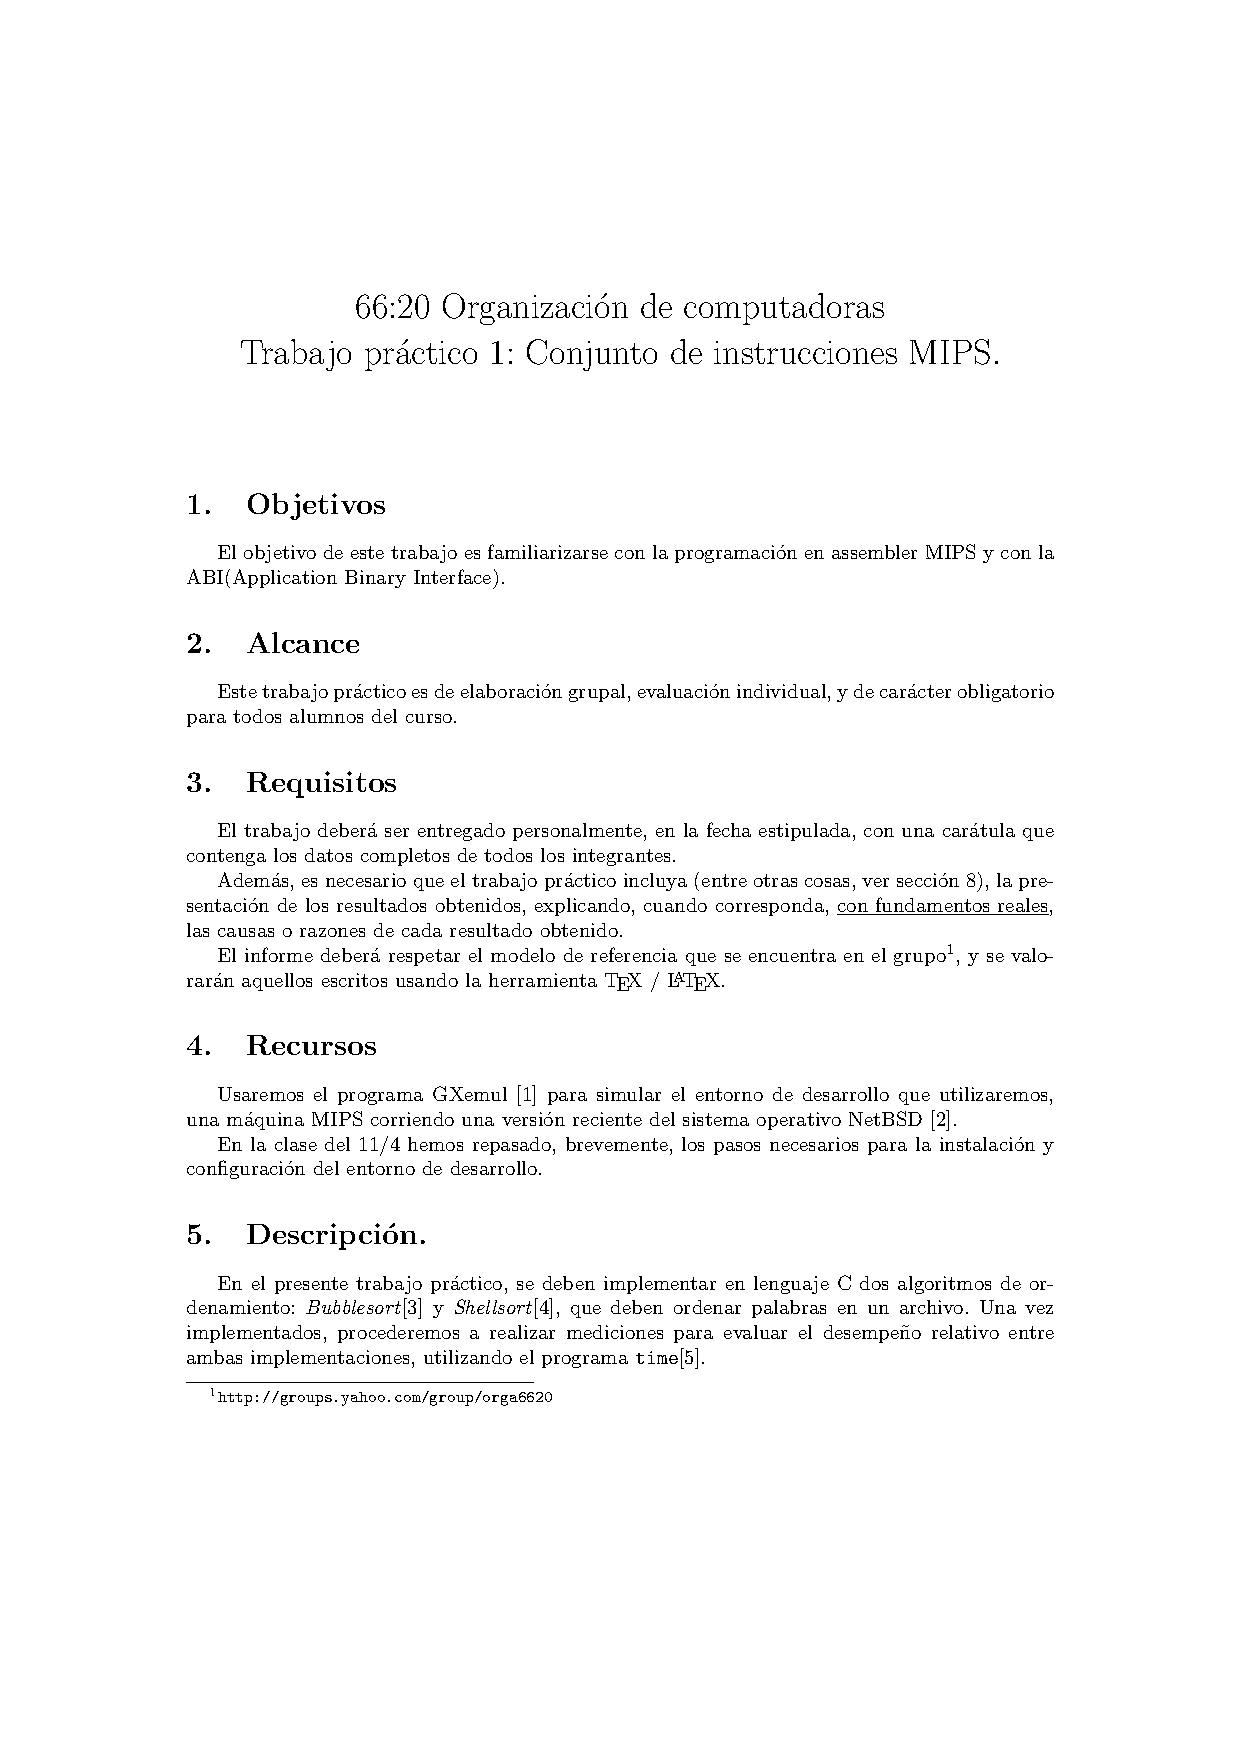
\includepdf[pages={-}]{docs/enunciado.pdf}

\clearpage
\section{README del material digital}\label{sec:readme}
\includepdf[pages={-}]{build/doc/README.pdf}

\clearpage
\section{Código fuente}\label{sec:source}
\clearpage
\definecolor{gray}{rgb}{0.5,0.5,0.5}
\lstset{
  title=\lstname,
  basicstyle=\footnotesize,
  showspaces=false,
  showstringspaces=false,
  breaklines=true,
  commentstyle=\color{gray},
  numbers=left,
  numberstyle=\tiny\color{gray},
  numbersep=5pt,
  frame=single
}

%\lstinputlisting{source/shellsort.h}
%\lstinputlisting{source/shellsort.S}

\end{document}
